% !TeX root = ../main.tex

\chapter{相关技术理论}

本章节主要介绍了系统实现和使用过程中所需的相关技术。首先作为web端系统平台,需要使用SpringBoot、
MyBatis、Mysql等后台开发技术。同时,数据湖分析系统作为大数据管理平台,数据仓库、
数据湖架构以及相关的开源技术组件,其中包括传统离线数仓架构、实时数仓架构、数据湖架构和相关的
开源技术组件。下面对相关技术进行简要介绍。

\section{后台开发相关技术}

基于Iceberg的数据湖分析系统使用的到的后台开发技术包括后端框架、持久化框架、关系型数据库等。

\subsection{SpringBoot}

基于Iceberg的数据湖分析平台采用SpringBoot作为后端开发框架\cite{21,41}。
SpringBoot是一款基于Spring框架的快速开发、微服务架构的开源框架。
它旨在简化Spring应用的初始化过程,降低学习曲线和开发成本,使开发
人员能够更加专注于业务逻辑的实现。SpringBoot具有以下优点:

(1)快速开发

SpringBoot提供了许多现成的开箱即用的组件和插件,这些组件和插件能够快
速地搭建起整个应用程序的基础架构,使得开发人员能够快速构建出可运行的应用。
同时,SpringBoot内置的Tomcat、Jetty等服务器也使得应用程序的部署变得简单快捷。
这样可以大大缩短开发周期,提高开发效率。

(2)简化配置

SpringBoot采用了"约定优于配置"的思想,大多数情况下,只需要通过少量的
配置就能完成应用的构建和部署。SpringBoot的自动化配置机制使得应用程序
的配置变得更加简单,开发人员不再需要手动配置复杂的XML文件。此外,SpringBoot
也支持注解配置,能够更加方便地完成配置工作。

(3)易于集成

SpringBoot与许多常用的技术和框架都有良好的集成能力,如Spring Data JPA、
Spring Security、Spring Cloud等。这意味着在使用SpringBoot时,开发人员
不需要对其他框架的配置和使用有过多的了解,只需要按照指导进行集成,就可以方便地
使用这些框架的功能。同时,由于SpringBoot本身就是基于Spring框架开发的,与Spring框架的整合也非常自然。

(4)可维护性高

SpringBoot提供了可视化的监控工具,可以通过监控工具查看应用程序的状态和性能。
这使得开发人员能够更加方便地进行应用程序的维护和优化。同时,SpringBoot还提
供了可扩展性良好的插件机制,可以方便地扩展应用程序的功能。

(5)良好的社区支持

SpringBoot拥有庞大的社区支持,官方提供了详细的文档和示例,社区也提供了大量
的插件和第三方库。这使得开发人员可以更加方便地使用和学习SpringBoot,同时也
能够及时地获取支持和帮助。

综上所述,SpringBoot具有快速开发、简化配置、易于集成、可维护性高和良好的社区
支持等优点,这些特点使得它成为企业级应用程序开发的首选框架。基于以上综合考虑,选择SpringBoot作为后端框架。

\subsection{MyBatis}

MyBatis是一个Java持久层框架,它可以轻松地将Java对象映射到数据库表中,并提供了许多高级功能,
如缓存和延迟加载\cite{21,22}。MyBatis具有以下优点:

(1)简单易学

MyBatis提供了一组简单易懂的API,使得开发人员可以很快地学会如何使用它。
与其他ORM框架相比,MyBatis的学习曲线较为平缓,使得新手也可以快速掌握。

(2)灵活性

MyBatis具有很高的灵活性。开发人员可以使用自己的SQL语句,而不是通过ORM框架生成的SQL语句。
这意味着开发人员可以编写自己的复杂SQL查询,以及使用数据库的高级功能。

(3)易于维护

MyBatis的Mapper XML文件是易于维护的。由于这些文件包含了所有的SQL查询语句,
所以开发人员可以很容易地修改它们。另外,这些文件的格式清晰明了,使得代码更加易于维护。

(4)性能优越

MyBatis具有很高的性能。由于开发人员可以直接使用原生SQL语句,所以MyBatis生成
的SQL语句更加紧凑和高效。此外,MyBatis提供了一些高级功能,如缓存和延迟加载,可以进一步提高性能。

(5)易于集成

MyBatis与其他框架的集成非常容易。它可以与Spring和Spring Boot等流行的框架无缝集成,使得开发人员可以快速地集成到现有的应用程序中。

总之,MyBatis是一个功能强大、易于学习和使用、灵活性高、易于维护、性能优越、
易于集成的持久层框架。基于以上综合考虑,我们选择了MyBatis。

\subsection{Mysql}

MySQL是一种开源的关系型数据库管理系统,它是目前最流行的数据库之一\cite{42}。MySQL的优点包括以下几个方面:

(1)可扩展性

MySQL具有高度可扩展性,它可以轻松地扩展到大型数据库系统。用户可以使用多个MySQL服务器进行集群配置,以实现更高的性能和可靠性。

(2)高性能

MySQL的性能非常出色,它可以处理大量的数据请求。此外,MySQL可以在多个平台上运行,包括Windows、Linux、Unix等操作系统。

(3)安全性

MySQL提供了一系列安全性功能,可以帮助保护数据库免受黑客和恶意软件的攻击。这些功能包括访问控制、加密、日志记录等。

(4)可靠性

MySQL是一种非常可靠的数据库系统,可以保证数据的完整性和一致性。MySQL提供了
事务支持和数据备份和恢复功能,确保即使在系统崩溃或其他意外情况下,数据也能够得到恢复。

(5)易于使用

MySQL拥有简单易用的界面和语法,用户可以快速上手使用。此外,MySQL拥有大量的文档和社区支持,用户可以通过互联网轻松获得帮助和支持。

总之,MySQL是一款强大而又灵活的数据库系统,它的可扩展性、高性能、安全性、可靠性和
易用性使它成为了业界标准之一。无论是中小型企业还是大型企业,都可以考虑使用MySQL来
管理和存储数据。

\section{传统离线数仓架构}

传统离线数据仓库(Offline Data Warehouse)是一种数据处理和存储方案,用于解决大型企业需要处理和分析大量数据的问题。
它由多个组成部分构成,包括数据源、ETL(Extract-Transform-Load)工具、数据存储和数据分析工具等\cite{27}。

(1)数据源

数据源是指从企业各个系统中收集和提取数据的来源。数据源可能包括企业内部的各种应用程序、
数据文件和日志文件等。这些数据源的格式和结构可能非常不同,需要经过ETL工具进行预处理,使其符合数据仓库的规范和标准。

(2)ETL工具

ETL是数据仓库中的一个关键环节,负责从数据源中提取数据、转换数据格式和结构、清洗数据,
最终将数据加载到数据仓库中。

(3)数据存储

数据存储是指用于存储和管理数据的硬件和软件设施,包括数据库、文件系统和分布式文件系统等。

(4)数据分析工具

数据分析工具是指用于从数据仓库中提取、分析和报告数据的工具和软件。
这些工具包括OLAP(Online Analytical Processing)、数据挖掘、报告和可视化工具等。

在传统离线数据仓库的架构中,数据源通过ETL工具进行预处理和转换,最终将数据存储在数据存储中。
数据分析工具可以从数据存储中提取和分析数据,并生成报告和可视化结果,以帮助企业做出决策和制定战略。

\section{实时数仓架构}

随着大数据应用的发展,人们对系统的实时性要求越来越高,对于传统离线数仓,
数据从接入直到展示存在着小时级以上的延迟\cite{25},这其中一方面是因为批处理框架本身延迟的限制,另一方面也是因为对于变化数据捕捉能力的缺失:

(1)无法避免的架构延迟

当前数仓的ETL入库过程通常是基于批的方式,数据按小时、天等的粒度导入到数据仓库中,
由于ETL的复杂度和固有的延迟,导致端到端的时延被放大到T+1;
数仓构建中的层次化划分和处理——原始层、明细层、汇总层、应用层——也在一定程度上增加了最后数据展示的延迟。

(2)高昂的数据修改成本

对于延迟数据的修正,以及近似数据的修正在传统的基于Hive的数仓中是一个非常高代价的操作,
Hive需要将相应的分区或文件读出来更新后重新写回到表中(即使只有一行数据的修改),而这在无形中也加剧了整体的时延。

为了解决现有离线数仓架构的问题,业界也在该领域进行了较多的探索,其中最主要的探索是Lambda架构和Kappa架构。

\subsection{Lambda 架构}

Lambda架构是一种常见的数据处理体系结构,
它使用两个计算层:流式计算层和批处理计算层,以处理数据。每隔数小时,批处理计算层会被触发,
以计算准确的业务状态,并将结果加载到服务层。同时,流式计算层用于实时更新业务数据,
但其结果只是近似值,需要被批处理计算覆盖\cite{3}。Lambda架构图如图\ref{fig:Lambda架构图}所示。

\begin{figure}[H]
  \centering
  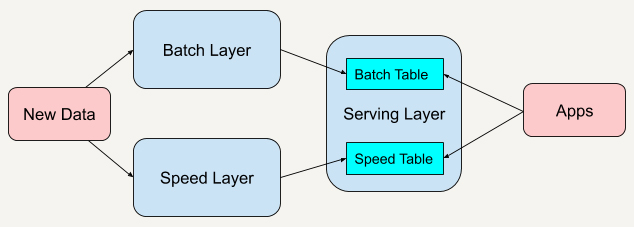
\includegraphics[width=1.0\textwidth]{Lambda.png}
  \caption{Lambda架构图}
  \label{fig:Lambda架构图}
\end{figure}

可以看到,为了实现近实时计算,需要设计复杂的架构,包括维护流式计算层和批处理计算层两种框架。
这两种框架之间的差异性导致了高昂的维护成本,同时,也需要维护不同的代码来服务这两种应用,
增加了开发和维护成本。此外,批处理和流处理的状态差异也需要提供不同的服务层,并在其上进行
合并抽象或设计相当复杂的服务系统。最后,由于数据存在于多个不同的源中,还可能导致数据不一致。

为了解决Lambda架构的复杂性,也出现有了诸多的改进方案,比如Kappa架构及其变种。

\subsection{Kappa 架构}

现有的流式框架和消息中间件可以快速增加并行度和处理历史数据以重新处理实时数据,
避免在实时数据处理系统中添加离线数据处理系统。因此提出了Kappa架构\cite{4}。

Kafka或其他消息中间件可以保留多日数据。通常,实时数据会被传输到实时处理系统,
然后存储在服务数据库中。如果需要订正数据,可以通过重放消息来修正实时处理代码,
并通过增加并发度扩展实时处理系统,从而快速回溯历史数据。Kappa架构图如图\ref{fig:Kappa架构图}所示。

\begin{figure}[H]
  \centering
  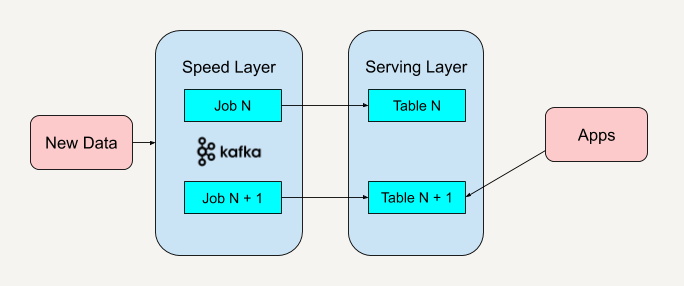
\includegraphics[width=1.0\textwidth]{Kappa.png}
  \caption{Kappa架构图}
  \label{fig:Kappa架构图}
\end{figure}

可以看到,该架构简单,避免了维护两套系统并保持结果一致的问题,同时也解决了数据订正问题。
然而,该架构也存在一些问题。首先,消息中间件缓存的数据量和回溯数据会存在性能瓶颈。例如,
如果算法需要过去180天的数据,而这些数据都存在于消息中间件中,那么对实时计算的资源消耗将非常大。
其次,在处理大量不同的实时流进行关联时,该架构非常依赖实时计算系统的能力。由于数据流的先后顺序问题,可能会导致数据丢失。

\section{数据湖架构}

数据湖是一种数据存储和处理架构,旨在容纳各种类型、格式和规模的原始数据\cite{12,14}。它与传统的数据仓库相比,具有更大的灵活性和可扩展性\cite{28,29}。
数据湖架构由以下几个主要组件构成:

(1)数据存储

数据湖可以使用云存储服务(如Amazon S3,Azure Blob Storage等)或者HDFS来存储原始数据。
数据以其原生格式存储,而不是被结构化为关系型数据库中的表格。

(2)数据采集

数据湖需要数据采集工具将数据从各种来源(例如应用程序、日志文件、数据库等)收集到数据湖中。

(3)数据标准化

在数据湖中,数据通常是以其原始格式存储,因此需要对数据进行标准化处理,以确保数据可被分析和查询。
这通常涉及将数据转换为常用格式(如JSON或CSV),并为每个数据元素添加描述信息。

(4)元数据管理

数据湖需要对存储在其中的数据进行元数据管理,以便能够有效地查询和分析数据。
元数据可能包括数据源、数据类型、数据格式、数据拥有者、数据质量等信息。

(5)数据访问

数据湖需要提供一种可扩展的机制,使用户能够方便地访问和查询数据。
通常使用查询服务(如Flink、Spark、Presto等)来实现数据访问。

(6)数据分析

数据湖支持各种数据分析工具和技术,例如机器学习、数据挖掘、自然语言处理等。
这些工具可以直接在数据湖中进行分析和处理,无需先将数据复制到其他位置。

总之,数据湖架构为企业提供了一种灵活、可扩展和可管理的方式,以存储、管理和分析大规模的原始数据。

\section{相关开源技术组件}

本小节主要介绍和本系统构建相关的几个核心开源组件,除了下述讨论的几个组件外,本系统在实现或者使用中
还涉及到了Hadoop、Presto、Parquet、Hive、Kafka、Flink CDC等大数据体系中常见的开源技术组件,因篇幅所限,
这里不再一一展开讨论。

\subsection{Apache Iceberg}

随着数据湖在大数据领域的流行,越来越多的公司开始使用Iceberg搭建统一的湖仓平台。
Iceberg是一种表格式(Table Format),我们可以简单理解为它是基于计算层(Flink、Spark)
和存储层(Orc\cite{9}、Parquet\cite{10})的一个中间层,我们可以把它定义成一种"数据组织格式",
Iceberg将其称之为"表格式"也是表达类似的含义。

数据格式顾名思义就是数据的存储格式。在大数据领域,随着对于性能的追求,
数据格式也在不停地进化,从TXT File,CSV File,Json File,Sequence File
等行式存储格式,到后期的RCFile,Parquet,ORC等列式存储格式。它们所表示的是在一个文件中数据是如何存储的。
在整个大数据软件栈中,Data Format所处的位置如图\ref{fig:DataFormat}如所示:

\begin{figure}[H]
  \centering
  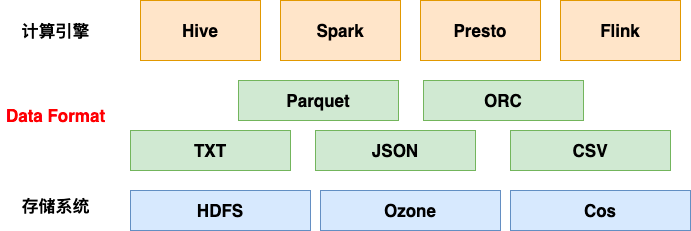
\includegraphics[width=1.0\textwidth]{DataFormat.png}
  \caption{Data Format示意图}
  \label{fig:DataFormat}
\end{figure}

数据格式所表示的是一个文件中数据的存储格式,而对于一张Hive表来说,它通常包含了多个文件,为了更好地利用HDFS\cite{13}这样的分布式文件系统进行文件过滤,
Hive表利用目录的方式来组织表:一张表映射到HDFS上是一个目录,目录中可以包含子目录,而子目录的定义是分区信息,
数据按分区列写入到不同的目录中,查询引擎据分区条件找到相应的目录。因此说,"以目录的方式来组织数据成为一张表"
是一种较为朴素的表组织方式,称为表格式。
而Iceberg的出现,试图打破现在这种朴素的表组织方式,定义了一种非目录形式的表组织方式,Table Format所处的位置如图\ref{fig:TableFormat}如所示:

\begin{figure}[H]
  \centering
  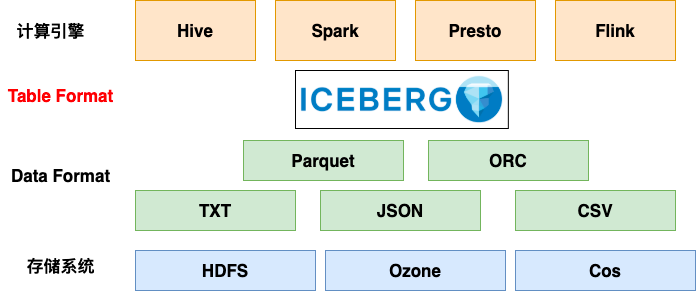
\includegraphics[width=1.0\textwidth]{TableFormat.png}
  \caption{Table Format示意图}
  \label{fig:TableFormat}
\end{figure}

因此,Iceberg是一种表格式,Iceberg定义了表中文件的组织方式,而不是一个文件中数据的格式;
是一个库,Iceberg是一个库,通过和计算引擎一起运行将表以Iceberg的组织方式写入到底层存储系统中\cite{26}。而不是一个独立的服务(不涉及部署);
是一个开放标准,Iceberg定义了一个开放的表格式,并在其上设计了一套引擎无关的API,因此任何引擎只要适配了Iceberg的API都可以读写Iceberg表。

\subsection{Apache Flink}

Apache Flink是一个分布式数据处理引擎,它提供了高效的流式计算和批处理功能。
Flink最初是为了解决流式数据处理的需求而设计,但它也能够支持离线批处理作业\cite{24}。
Flink的主要优点包括:

(1)低延迟处理

Flink是一个实时数据处理引擎,能够在毫秒级别内对数据进行处理,具有非常低的延迟。

(2)高吞吐量

Flink的流处理引擎能够处理大量的数据,并支持多种数据源和格式。

(3)灵活性

Flink支持多种计算模式,包括批处理、流处理和迭代计算,这使得它非常适合处理各种类型的数据处理任务。

(4)可扩展性

Flink的架构设计使其可以轻松地水平扩展,可以根据需要添加更多的计算节点以提高处理能力。

(5)稳定性和容错性

Flink能够在节点故障或其他异常情况下自动恢复,并保证计算结果的准确性。

总之,Apache Flink是一个功能强大、灵活性高、性能优秀的分布式数据处理引擎,
可以帮助用户轻松地进行各种类型的数据处理任务,包括流式计算、批处理、迭代计算等。

\subsection{Apache Spark}

Apache Spark是一个快速、通用、分布式的计算引擎,它能够在大规模数据集上执行数据处理和分析任务。
Spark最初是为了解决Hadoop批处理任务的瓶颈问题而设计,但它也能够支持流式计算、机器学习、
图形计算等多种数据处理任务\cite{23}。Spark的主要优点包括:

(1)高速处理

Spark采用了内存计算模式,能够在内存中进行计算,因此比Hadoop MapReduce等传统计算引擎快很多。

(2)多种计算模式

Spark支持多种计算模式,包括批处理、流式处理、机器学习等,能够处理各种类型的数据处理任务\cite{43}。

(3)易用性

Spark提供了Python、Scala、Java等多种编程语言的API,以及丰富的开发工具和调试工具,使得开发者可以更轻松地使用Spark进行数据处理。

(4)可扩展性

Spark能够轻松地水平扩展,可以根据需要添加更多的计算节点以提高处理能力。

(5)兼容性

Spark可以与多种数据源和存储系统(如HDFS、Iceberg、HBase等)集成,可以处理不同格式和类型的数据。

总之,Apache Spark是一个强大、易用、高性能的分布式计算引擎,能够处理各种类型的数据处理任务,
包括批处理、流式处理、机器学习等。Spark的快速处理能力、多种计算模式、可扩展性和兼容性使得它成为了数据处理领域中广泛使用的工具。

\subsection{Hive Metastore}

Hive Metastore是Hive的一个组件,它是元数据的存储和管理系统,
可以用于管理Iceberg表的的分区、列等元数据信息。Hive Metastore支持多种元数据存储方式,
如MySQL、HDFS等,开发者可以根据需要选择合适的元数据存储方式\cite{30}。
Hive Metastore具有以下主要功能:

(1)元数据存储

Hive Metastore负责将Iceberg表的元数据信息存储在关系型数据库或文件系统中,包括表、分区、列等元数据信息。

(2)元数据管理

Hive Metastore提供了对Iceberg表元数据的管理功能,包括表的创建、删除、重命名、分区的添加、删除、修改等。

(3)元数据查询

Hive Metastore提供了元数据查询的API,可以查询Iceberg表、分区、列等元数据信息。

(4)权限管理

Hive Metastore可以通过配置元数据存储和使用的权限,实现对Iceberg元数据的访问控制。

(5)集成

Hive Metastore可以与其他Hadoop生态系统中的组件集成,如Hadoop、Spark等。

总之,Hive Metastore是管理元数据的一个重要组件,可以用于存储和管理Iceberg表的元数据信息,
支持多种元数据存储方式,提供了元数据管理、查询、权限管理等功能,使得开发者可以更加方便地进行数据处理和分析。

\section{本章小结}

本章主要对数据湖分析系统在实现以及使用过程中用到的关键技术进行介绍。首先介绍了后台系统开发使用到的技术,包括SpringBoot、
MySQL等,然后介绍了传统离线数仓模型、实时数仓模型、数据湖模型,最后介绍了相关的开源技术组件,这为后续的讨论打下了理论基础。
因篇幅有限,故而只讨论了几个比较核心的组件,后文将这些技术有机整合在一起,形成新一代的全场景实时数仓——数据湖分析系统。
